\documentclass{book} 
\usepackage{commeunjeustyle} 

\begin{document}

\chapter*{Topologie des espaces vectoriels normés}

Ce cours présente les grands concepts à l'origine de la topologie et de l'analyse fonctionnelle.
L'étymologie du mot "topologie" est éloquente. En effet, en Grec, topos signifie lieu tandis que
logos signifie étude. Ce domaine des Mathématiques s'intéresse donc à l'étude des lieux, appelés en général espaces et
aux propriétés qui les caractérisent.\\
La chronologie adoptée pour écrire ce cours complet n'est pas logique. Pour une cohérence mathématiques, il faudrait étudier d'abord ce chapitre avant les chapitres d'analyse ou d'algèbre. \\
Cependant, ce chapitre décourage de nombreux élèves dès le début d'année du fait de son caractère abstrait. C'est pourquoi d'un point de vue  pédagogique, il est étudier à la fin.\\
Les résultats de la topologie de première année sont  :  la définition de la convergence
d'une suite réelle, la notion d'intervalle ouvert (notion qui intervient dans le théorème de Rolles) ou d'intervalle fermé (notion qui intervient 
théorème "si $f$ est continue sur un intervalle fermé borné, à valeurs dans $\R$, alors f admet un minimum et un maximum »).\\
Le problème est de généraliser les notions de topologie sur la droite des réels à d'autres ensembles, par exemples les points du plan, les polynômes, les fonctions continues...  Quelle serait la définition d'un intervalle ouvert dans le plan ? \\
Dans le cadre de ce cours, on limite l'abstraction à une topologie définie à partir d'une norme. Une norme est un objet mathématique donnant du sens à la notion de "longueur".\\
Dans tout le chapitre, $\K$ désigne $\R$ ou $\C$.


% -----------------------------------------------------------------------------
\section{Espace vectoriel normé}

\subsection{Norme}
En géométrie, la norme est une extension de la valeur absolue des nombres aux vecteurs. Elle permet de mesurer la longueur commune à toutes les représentations d'un vecteur.
\begin{Definition}[Norme]
Soit $E$ un $\K$-espace vectoriel.\\
Une \defi{norme} sur $E$ est une application $N:E\to\R$ vérifiant les axiomes suivants.
%Pour tous $(x,y)\in E^2$ et pour tout $\lambda  \in \K $:
\begin{enumerate}
\item \defi{positivité :} $\forall \vec{x}\in E:\quad N(\vec{x})\geq 0$
\item \defi{définie :} $\forall \vec{x}\in E:\quad N(\vec{x}) = 0 \implies \vec{x} = \vec{0_E}$
\item \defi{homogénéité :} $\forall \vec{x}\in E,\forall\lambda\in\K:\quad N(\lambda  \vec{x}) = |\lambda| N(\vec{x})$
\item \defi{inégalité triangulaire :} $\forall \vec{x},\vec{y}\in E:\quad N(\vec{x}+\vec{y}) \leq  N(\vec{x}) + N(\vec{y})$
\end{enumerate}
On note fréquemment $\norme{\vec{x}}$ au lieu de $N(\vec{x})$.\\
La norme d'un vecteur correspond à sa "longueur".
\end{Definition}
\begin{Remarque}
Une conséquence des axiomes précédent est que $N(\vec{0}) = 0$ (en appliquant 3) avec $\lambda= 0$.\\
        \begin{minipage}[c]{0.45\linewidth}{
Le nom d'inégalité triangulaire vient du fait que dans un triangle $ABC$ on a nécessairement $$AC \leq AB + BC.$$}
\end{minipage}
    \begin{minipage}[c]{0.45\linewidth}{
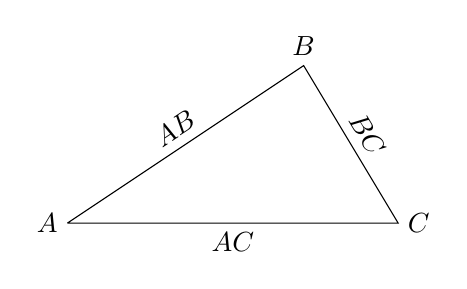
\begin{tikzpicture}[scale=1]%,cap=round,>=latex]
   \coordinate [label=left:$A$] (A) at (-2cm,-1.cm);
   \coordinate [label=right:$C$] (C) at (2.2cm,-1.0cm);
   \coordinate [label=above:$B$] (B) at (1cm,1.0cm);
   \draw (A) -- node[sloped,above] {$AB$} (B) -- node[sloped,above,] {$BC$} (C) -- node[below] {$AC$} (A);
\end{tikzpicture}}
    \end{minipage}
\end{Remarque}
\begin{Definition}[Espace vectoriel normé]
Un \defi{espace vectoriel normé} est un couple $(E,N)$ où $E$ est un espace vectoriel et $N$ un norme sur $E$.
On note parfois $E$ au lieu de $(E,N)$ si le choix de la norme est clair d'après le contexte.
\end{Definition}
\begin{Proposition}[Inégalité triangulaire inversée]
Soit $E$ un espace vectoriel, $N$ une norme sur $E$. On a :
$$\vec{x},\vec{y}\in E: |N(\vec{x}) - N(\vec{y})|\leq N(\vec{x}-\vec{y}).$$
\end{Proposition}
\begin{Demonstration}
Soit $\vec{x},\vec{y}\in E$. On a $$N(\vec{x})=N(\vec{x}-\vec{y}+\vec{y})\overbrace{\leq}^{\text{inégalité triangulaire}} N(\vec{x}-\vec{y})+N(\vec{y}).$$
Ainsi $N(\vec{x})-N(\vec{y})\leq N(\vec{x}-\vec{y}).$ En permutant $\vec{x}$ et $\vec{y}$, on obtient $N(\vec{y})-N(\vec{x})\leq N(\vec{x}-\vec{y}).$ Finalement $|N(\vec{x}) - N(\vec{y})|\leq N(\vec{x}-\vec{y}).$
\end{Demonstration}
\begin{Proposition}[Norme hilbertienne]
Soit $(E,\PS{}{})$ est un espace prehilbertien réel.
La \defi{norme associée} définie par 
$$ \forall \vec{x}\in E:\quad  \norme{\vec{x}} =\sqrt{\PS{\vec{x}}{\vec{x}}}.$$
est une norme sur $E$. 
\end{Proposition}

\begin{Exemple}[Trois normes sur $\K^n$]
Pour $\vec{x} =(x_1,\dots,x_n)\in \K^n$, on pose
\begin{enumerate}
\item $\norme{\vec{x}}_1 = \sum_{k=1}^n |x_k|$
\item $\norme{\vec{x}}_2 = \sqrt{\sum_{k=1}^n |x_k|^2}$
\item $\norme{\vec{x}}_\infty = \max\Big(|x_1|,\dots,|x_n|\Big)$
\end{enumerate}
Démontrons que $\norme{\,}_\infty$ est une norme sur $\K^n$. \\
\begin{itemize}
\item \textit{positivité :} le plus grand élément d'un nombre fini de réels positifs est lui-même un réel positif. 
\item \textit{définie :} Soit $\vec{x}=(x_1,\dots,x_n)\in \K^n$ tel que $\norme{\vec{x}}_\infty=0$. On a :
 $$\forall i\in \Intf{1}{n} :\quad  0\leq |x_i|\leq \norme{\vec{x}}_\infty=0.$$ Donc pour tout $i\in\Intf{1}{n},x_i=0$, soit  $\vec{x}=\vec{0}$.
\item \textit{homogénéité :} Soit $\vec{x}=(x_1,\dots,x_n)\in \K^n$ et $\lambda\in\K$.  Si $\lambda$ est nul, l'égalité cherchée est immédiate. On suppose $\lambda$ non nul.
On a :
$$\forall i\in \Intf{1}{n} : |\lambda x_i| = |\lambda| |x_i|\leq |\lambda| \norme{\vec{x}}_\infty.$$ Comme tous les termes sont majorés par une même constante, on en déduit que  $  \norme{\lambda\vec{x}}_\infty \leq |\lambda| \norme{\vec{x}}_\infty$.\\
On a aussi :
$$\norme{\vec{x}}_\infty=\norme{\frac{1}{\lambda}\lambda\vec{x}}_\infty\leq \frac{1}{|\lambda|} \norme{\lambda\vec{x}}_\infty.$$
 et on obtient ainsi une deuxième inégalité, puis l'égalité voulue. 
\item \textit{inégalité triangulaire :} Soit $\vec{x}=(x_1,\dots,x_n),vec{y}=(y_1,\dots,y_n)\in \K^n$.
$$\forall i\in \Intf{1}{n} :\quad  0\leq |x_i+y_i|\leq |x_i|+|y_i|\leq \norme{\vec{x}}_\infty +\norme{\vec{y}}_\infty .$$ Comme tous les termes sont majorés par une même constante, on en déduit que  $  \norme{\vec{x}+\vec{y}}_\infty \leq  \norme{\vec{x}}_\infty+\norme{\vec{y}}_\infty$.
\end{itemize}  

\end{Exemple}


\begin{Exemple}[Trois normes sur les espaces de fonctions]
\begin{itemize}
\item Soit $\mathcal{B}(I, \K)$ l'espace des fonctions bornées sur l'intervalle I de $\R$ à valeurs dans $\K$.  Pour $f \in  \mathcal{B}(I, \K)$, on pose :
$$\norme{f}_\infty=\sup_{x\in I}|f(x)|.$$
$\norme{\,}_\infty$ est une norme sur $\mathcal{B}(I, \K)$ appelée \defi{norme de la convergence uniforme.}
\item Soit $L_1(I, \K)$ l'espace des fonctions continues et intégrables sur l'intervalle $I$ de $\R$ à valeurs dans $\K$. Pour $f \in L_1(I, \K)$, on pose :
$$\norme{f}_1=\int_I|f(x)|\,\mathrm{dx}.$$
$\norme{\,}_1$ est une norme sur $L_1(I, \K)$ appelée \defi{norme de la convergence en moyenne.}
\item Soit $L_2(I, \K)$ l'espace des fonctions continues de carré intégrables sur l'intervalle $I$ de $\R$ à valeurs dans $\K$. Pour $f \in L_2(I, \K)$, on pose :
$$\norme{f}_1=\sqrt{\int_I f^2(x)}\,\mathrm{dx}.$$
$\norme{\,}_2$ est une norme sur $L_2(I, \K)$ appelée \defi{norme de la convergence quadratique.}
Comme l'ensemble des fonctions continues sur un segment $[a,b]$ à valeurs dans $\K$, $\mathcal{C}([a,b],\K)$ est une partie des ensembles $\mathcal{B}(I, \K)$, $L_1(I, \K)$ et $L_2(I, \K)$, $\norme{\,}_\infty$, $\norme{\,}_1$ et $\norme{\,}_2$ sont trois normes de $\mathcal{C}([a,b],\K)$.
\end{itemize}
\end{Exemple}


\begin{Theoreme}[Norme équivalente en dimension finie]
Soit $E$ un espace vectoriel de dimension finie.\\
Soit $N_1$ et $N_2$ deux normes sur $E$.\\
Alors il existe deux réels strictement positifs $\alpha, \beta$ tel que 
$$\forall \vec{x}\in E : \alpha N_1(\vec{x})\leq N_2(\vec{x})\leq \beta N_1(\vec{x}).$$ 
\end{Theoreme}
\begin{Exemple}[$\R^n$]  
Pour les normes $\norme{\,}_\infty$ et $\norme{\,}_1$, on peut déterminer les constantes $\alpha, \beta$. On a  $$\forall \vec{x}\in E :  \norme{\vec{x}}_\infty\leq \norme{\vec{x}}_1 \leq n \norme{\vec{x}}_\infty.$$
En effet, soit $\vec{x}=(x_1,\dots,x_n)\in \R^n$, d'une part :
$$\norme{\vec{x}}_1=\sum_{i=1}^n |x_i|\leq \sum_{i=1}^n \norme{\vec{x}}_\infty=n\norme{\vec{x}}_\infty$$
et d'autre part, soit $i_0$ l'indice tel que $\norme{\vec{x}}_\infty = |x_{i_0}|$,
$$\norme{\vec{x}}_\infty=|x_{i_0}|\leq \sum_{i=1}^n |x_i| =  \norme{\vec{x}}_1.$$
\end{Exemple}
\subsection{Distance}
\begin{minipage}[c]{0.6\linewidth}{
Une distance est une application qui formalise l'idée intuitive de distance, c'est-à-dire la longueur qui sépare deux vecteurs.}
\end{minipage}
    \begin{minipage}[c]{0.4\linewidth}{
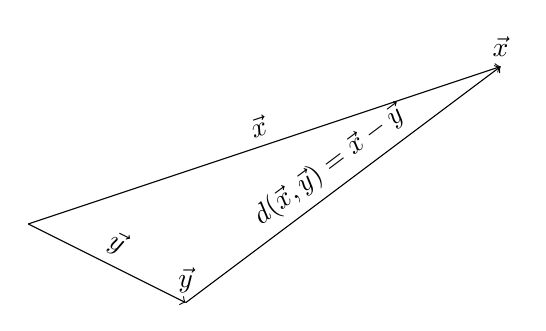
\begin{tikzpicture}
   \coordinate [label=above:$\vec{x}$] (A) at (6,2);
   \coordinate   (0) at (0,0);
   \coordinate [label=above:$\vec{y}$] (B) at (2,-1);
   \draw[->] (0) -- node[sloped,above] {$\norme{\vec{x}}$} (A);
   \draw[->] (0) -- node[sloped,above] {$\norme{\vec{y}}$} (B);
   \draw[->] (B) -- node[sloped,above] {$d(\vec{x},\vec{y})=\norme{\vec{x}-\vec{y}}$} (A);
\end{tikzpicture}}
    \end{minipage}
\begin{Definition}
Soit $(E,\norme{\,})$ un espace vectoriel normé.\\
Pour tout $\vec{x},\vec{y}\in E$, la \defi{distance} de $\vec{x}$ à $\vec{y}$ est : 
$$d(\vec{x},\vec{y}) = \norme{\vec{x}-\vec{y}}.$$
\end{Definition}

\begin{Remarque}[Distance]
La notion de distance permet de définir la notion de convergence d'une suite $(\vec{x_n})_{n\in\N}$ vers $\vec{x}$. La convergence est l'idée que les éléments de la suite s'approche de plus en plus $\vec{x}$ quand $n$ augmente, c'est à dire que la distance entre $\vec{x_n}$ et $\vec{x}$ tend vers zero quand $n$ tend vers l'infini, soit $d(\vec{x_n},\vec{x})\tend[n\to\infty]0.$ 
\end{Remarque}
\begin{Proposition}
Ainsi définie, la distance vérifient les propriétés suivantes :
\begin{enumerate}
\item \defi{positivité :} $\forall \vec{x},\vec{y}\in E:\quad  d(\vec{x},\vec{y}) \geq  0$
\item \defi{symétrie :} $\forall \vec{x},\vec{y}\in E:\quad d(\vec{x},\vec{y}) = d(\vec{y},\vec{x})$
\item \defi{séparation :} $\forall \vec{x},\vec{y}\in E:\quad  d(\vec{x},\vec{y}) = 0 \Rightarrow \vec{x} = \vec{y}$
\item \defi{inégalité triangulaire :} $\forall \vec{x},\vec{y},\vec{z}\in E:\quad  d(\vec{x},\vec{y}) \leq d(\vec{x},\vec{z}) + d(\vec{z},\vec{y})$
\end{enumerate}
\end{Proposition}
\begin{Remarque}
La notion de distance est une notion mathématique qui est normalement définie à partir de cette liste de propriétés. La distance définie à partir d'un norme est un cas particulier de distance. 
\end{Remarque}
\begin{Definition}[Distance à une partie]
Soit $A$ partie non vide de $E$ et $\vec{x}\in E$.\\
La \defi{distance d'un point à une partie non vide} appelé distance de $x$ à $A$ est le réel positif ou nul
$$d (\vec{x}, A) = \inf_{\vec{a} \in A}  \norme{\vec{x} - \vec{a}}.$$
\end{Definition}


\subsection{Boules}
\begin{Definition}[Boule ouverte, boule fermé, sphère]
Soit $(E,\norme{\,})$ un espace vectoriel normé.
\begin{itemize}
\item La \defi{boule ouverte} de centre $\vec{a}\in E$ et de rayon $r\in \R $ est $$B(\vec{a},r) = \{\vec{x}\in E:\quad \norme{\vec{x}-\vec{a}}<r\}.$$
\item La \defi{boule fermée} de centre $\vec{a}\in E$ et de rayon $r\in \R $ est $$B_f(\vec{a},r) = \{\vec{x}\in E:\quad \norme{\vec{x}-\vec{a}}\leq r\}.$$
\item La \defi{sphère} de centre $\vec{a}\in E$ et de rayon $r\in \R $ est $$S(\vec{a},r) = \{\vec{x}\in E:\quad \norme{\vec{x}-\vec{a}}=r\}.$$
\end{itemize}
La \defi{boule unité ouverte}  est $B_f(\vec{0}, 1)$. La \defi{sphère unité} est l'ensemble des vecteurs de $E$ de
norme 1 ou encore l'ensemble des vecteurs unitaires de $E$.
\end{Definition}
\begin{Exemple}[Sphère unité dans $\R^2$]
Notons respectivement $S_1$, $S_2$, $S_{\infty}$ et $S_{\frac 1 2}$ les sphères unités de $\R^2$  muni de respectivement des normes $\norme{\,}_1,\norme{\,}_2,\norme{\,}_\infty,\norme{\,}_\frac{1}{2}$. \\
On identifie les coordonnées d'un vecteur avec les coordonnées d'un point du plan.
Le dessin des sphères est : \\
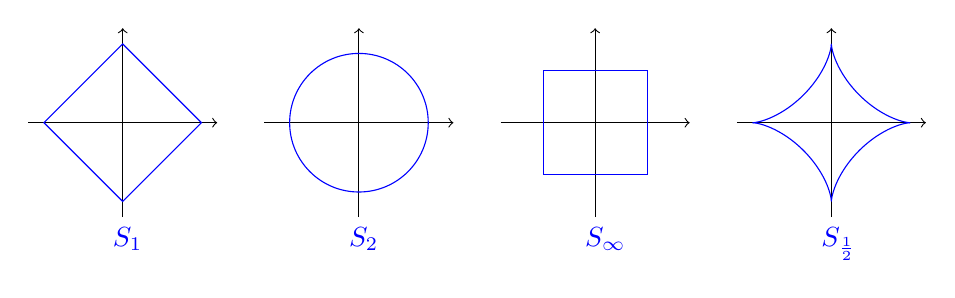
\begin{tikzpicture}
   \foreach \i in {0,...,3}{
     \begin{scope}[xshift=\i*3cm]
      \draw [->] (-1.2,0)--(1.2,0);
      \draw [->] (0,-1.2)--(0,1.2);
    \end{scope}
   }
   \begin{scope}[draw=blue,]
     \draw [] (-1,0)--(0,1)--(1,0)--(0,-1)--cycle;
     \draw [](3,0) circle (0.88cm);
     \draw [xshift=6cm] (-.66,-.66) rectangle (.66,.66);
     \begin{scope}[xshift=9cm]
       \draw [domain=0:90,samples=100,smooth,variable=\t] plot({-1*cos(\t)^(3)},{1*sin(\t)^(3)});
       \draw [domain=0:90,samples=100,smooth,variable=\t] plot({-1*cos(\t)^(3)},{-1*sin(\t)^(3)});
       \draw [domain=0:90,samples=100,smooth,variable=\t] plot({1*cos(\t)^(3)},{-1*sin(\t)^(3)});
       \draw [domain=0:90,samples=100,smooth,variable=\t] plot({1*cos(\t)^(3)},{1*sin(\t)^(3)});
     \end{scope}
   \end{scope}
   \foreach \i [count=\j from 0] in {1,2,\infty,\frac{1}{2}} \scoped [xshift=\j*3cm] { \node [anchor=mid west,color=blue] at (-0.25,-1.5) {$S_\i$}; };
\end{tikzpicture}.
\end{Exemple}
\begin{Remarque}Attention aux "faux-amis" !  On parle de boule ouverte associée à une norme,
bien qu'en général, une boule n'ait rien de rond. En effet, si l'on considère par exemple la norme $\norme{\,}_\infty$, la  la boule unité ouverte est un carré.
\end{Remarque}
\subsection{Partie convexe}
\begin{Definition}[Partie Convexe]
    \begin{minipage}[c]{0.4\linewidth}{
Soit $E$ un espace vectoriel et $A$ une partie de $E$.\\
On dit que $A$ est une \defi{partie convexe}, ou plus simplement que $A$ est \defi{convexe}, si  pour tous $\vec{x}$ et $\vec{y}$ de $A$, le segment $[\vec{x}, \vec{y}]$ est tout entier contenu dans $A$, c'est à dire
$$\forall \vec{x},\vec{y}\in A, \forall \lambda  \in [0,1]:\quad \lambda  \vec{x} + (1-\lambda)\vec{y}\in A.$$
}
\end{minipage} 
    \begin{minipage}[c]{0.6\linewidth}{
    \begin{center}
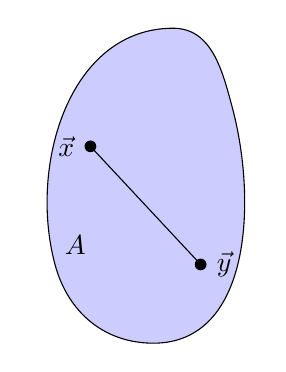
\begin{tikzpicture}[bullet/.style={circle,fill,inner sep=1.5pt,node contents={}}]

 \draw[black,fill=blue!20] (0,0) to[out=105,in=0] ++ (-0.75,1) to[out=180,in=105] ++ (-1.5,-3) node[above right]{$A$} to[out=-75,in=180] ++ (1.25,-1) to[out=0,in=-75] cycle;
 \draw (-1.8 ,-0.5) node[bullet,label=left:$\vec{x}$,alias=PC]--(-0.4,-2) node[bullet,label=right:$\vec{y}$];
\end{tikzpicture}
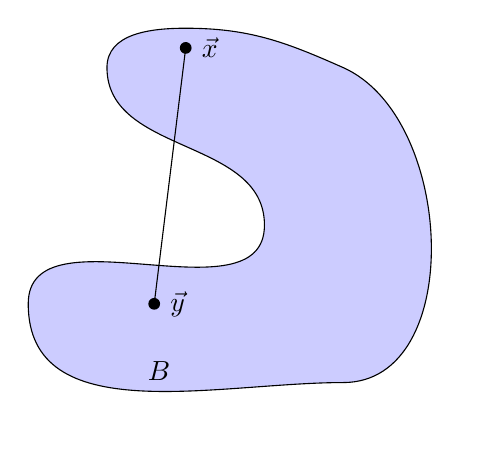
\begin{tikzpicture}[bullet/.style={circle,fill,inner sep=1.5pt,node contents={}}]
\pgfmathsetmacro{\myslope}{atan2(2,-4.5)}
\draw[fill=blue!20] (2,1) to[out=\myslope,in=0] ++ (-2,0.5)  to[out=180,in=90] ++ (-1,-0.5)
 to[out=-90,in=90] ++ (2,-2) to[out=-90,in=90] ++ (-3,-1)
 to[out=-90,in=180]node[above right]{$B$} ++(4,-1) to[out=0,in=\myslope+180] cycle;
  \draw (0 ,1.25) node[bullet,label=right:$\vec{x}$,alias=PC]--(-0.4,-2) node[bullet,label=right:$\vec{y}$];
\end{tikzpicture}\\
$A$ convexe. $B$ non convexe.
   \end{center}
}
\end{minipage} 
\end{Definition}
\begin{Proposition}[Convexité des boules]
    \begin{minipage}[c]{0.6\linewidth}{
Soit $(E,\norme{\,})$ un espace vectoriel normé.\\
Les boules ouvertes et fermés  sont convexes.}
\end{minipage} 
    \begin{minipage}[c]{0.3\linewidth}{
    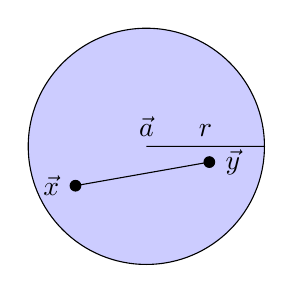
\begin{tikzpicture}[bullet/.style={circle,fill,inner sep=1.5pt,node contents={}}]
\draw [black,fill=blue!20]  (0,0) circle (1.5) (0,0)node[above]{ $\vec{a}$ } --(0:1.5)node[pos=0.5,above]{ $r$ };
\draw (-0.9 ,-0.5) node[bullet,label=left:$\vec{x}$]--(0.8,-0.2) node[bullet,label=right:$\vec{y}$];
\end{tikzpicture}
}
\end{minipage} 
\end{Proposition}
\begin{Demonstration}
Soit $B(\vec{a},r)$ une boule ouverte.\\
Soit $\vec{x},\vec{y}\in B(\vec{a},r).$ Soit $\lambda\in[0,1]$. On a :
$$ \norme{(\lambda \vec{x} + (1-\lambda)\vec{y})-\vec{a}   }=\norme{(\lambda(\vec{x}-\vec{a}) + (1-\lambda)(\vec{y}-\vec{a})   }\leq |\lambda|\norme{\vec{x}-\vec{a}}+|1-\lambda|\norme{\vec{y}-\vec{a}}< |\lambda|r+|1-\lambda|r\overbrace{=}^{\lambda\in[0,1]} r.$$
\end{Demonstration}
\begin{Exemple}
Les sous espaces vectoriels sont des convexes.
\end{Exemple}
\section{Suite vectorielle}
Dans cette partie, $(E,\norme{\,})$ désigne un espace vectoriel normé.
\subsection{Définition}
\begin{Definition}[Suite vectorielle]
Une \defi{suite vectorielle} est une application $\vec{x}:\N \to E$.\\
On note fréquemment le \defi{terme} $\vec{x_n}$ au lieu de $\vec{x}(n)$ pour représenter l'indexation par les entiers naturels.   Aussi, on note $(\vec{x_n})_{n\in\N}$ au lieu de $\vec{x}$.
\end{Definition}
\newpage
\begin{Exemple}[Suite de fonctions]
    \begin{center}
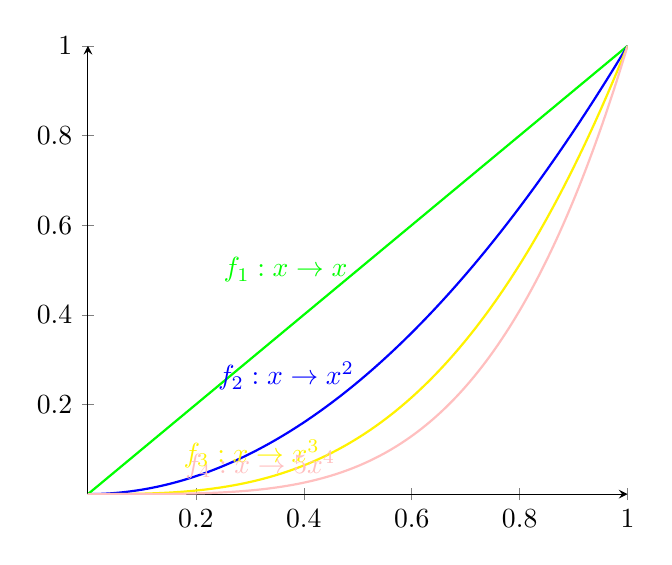
\begin{tikzpicture}
   \begin{axis}[
       axis y line = middle,
       axis x line = middle,
       samples     = 200,
       domain      = 0:1,
       xmin = 0, xmax = 1,
       ymin = 0, ymax = 1,
       unbounded coords=jump
     ]
     \addplot[green, thick, mark=none] {x}node[pos=0.5, left] {$f_1:x\to x$};
     \addplot[blue, thick, mark=none] {x^2}node[pos=0.4, left] {$f_2:x\to x^2$};
     \addplot[yellow, thick, mark=none] {x^3}node[pos=0.3,left] {$f_3:x\to x^3$};    
     \addplot[pink, thick, mark=none] {x^4}node[pos=0.2,above] {$f_4:x\to 5x^4$};
   \end{axis}
\end{tikzpicture}\\
Représentation graphique des premiers termes de la suite de fonctions $(f_n:x\to x^n)_{n\in \N   }$
\end{center}
\end{Exemple}


\subsection{Suite bornée}
\begin{Definition}[Suite bornée]
On dit que la suite $(\vec{x_n})_{n\in\N}$ est \defi{bornée} si il existe réel positif $M$ tel que :
$$\forall n \in \N:\quad \norme{\vec{x_n}}\leq M.$$
\end{Definition}
\begin{Remarque}[Dépendance de la norme en dimension infinie]
La notion de suite bornée est définie à partir d'une norme. Si on change de norme (et donc on change d'espace vectoriel
normé), il est possible que la suite considérée ne soit plus bornée.\\
En effet, soit la suite $(f_n)_{n\in\N}$ d'éléments $\mathcal{C}([0,1],\K)$ définie par $f_n:x\mapsto (n+1)x^n.$\\
On a :
\begin{itemize}
\item $\norme{f_n}_{1}=\int_0^1  |(n+1)x^n|\,\mathrm{dx}=1$, donc la suite  $(f_n)_{n\in\N}$ est une suite bornée de l'espace vectoriel normée $(\mathcal{C}([0,1],\K), \norme{\,}_1)$.
\item On a $\norme{f_n}_{\infty}=\sup_{x\in[0,1]}|(n+1)x^n|=(n+1)$. Puisque $\norme{f_n}_{\infty}\tend[n\to\infty]\infty$, la suite  $(f_n)_{n\in\N}$ n'est pas une suite bornée de l'espace vectoriel normée $(\mathcal{C}([0,1],\K), \norme{\,}_\infty)$.
\end{itemize}
\end{Remarque}






\subsection{Suite convergente}
De manière intuitive, la suite admet pour limite $\vec{l}$ (converge vers $\vec{l}$) quand les termes de la suite se rapprochent  vers cet élément limite, $\vec{l}$,  quand les indices deviennent très grands. Une définition plus rigoureuse est 
\begin{itemize}  
\item "se rapprochent"; quelque soit la rayon, noté $\epsilon$, les termes appartiennent à la boule centrée en $\vec{l}$ et de rayon $\epsilon$,
\item  "quand les indices deviennent très grands" : il existe un rang $N$ telle que cette propriété est vraie pour tous les indices à partir de ce rang. 
\end{itemize} 
\begin{center}
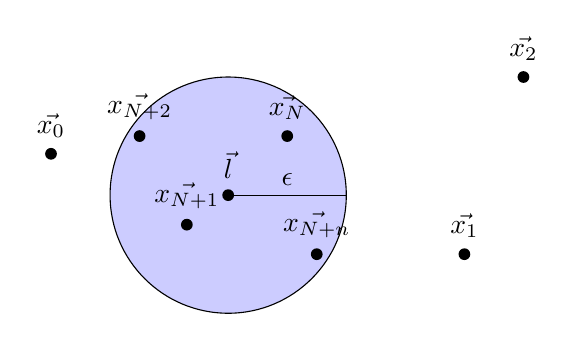
\begin{tikzpicture}[scale=0.75,bullet/.style={circle,fill,inner sep=1.5pt,node contents={}}]
\draw [black,fill=blue!20]  (0,0) circle (2);
\draw (0,0)node[bullet,label=above:$\vec{l}$] --(2,0)node[pos=0.5,above]{ $\epsilon$} ; 
\draw (1,1)node[bullet,label=above:$\vec{x_N}$]; 
\draw (-0.7,-0.5)node[bullet,label=above:$\vec{x_{N+1}}$];
\draw (-1.5,1)node[bullet,label=above:$\vec{x_{N+2}}$];
\draw (1.5,-1)node[bullet,label=above:$\vec{x_{N+n}}$];
\draw (-3,0.7)node[bullet,label=above:$\vec{x_{0}}$];
\draw (4,-1)node[bullet,label=above:$\vec{x_{1}}$];
\draw (5,2) node[bullet,label=above:$\vec{x_{2}}$];
\end{tikzpicture}\\
Exemple de suite dans $\R^2$. Quelque soit le rayon $\epsilon$, à partir d'un certain rang $N$, tous les termes de la suite doivent appartenir à la boule $B(\vec{l},\epsilon)$
\end{center}

\begin{Definition}[Convergence et limite]
On dit que la suite $(\vec{x_n})_{n\in\N}$ admet pour \defi{limite} $\vec{l}$ au sens de $\norme{\,}$ si :
$$\forall  \epsilon > 0,\overbrace{\exists N \in \N, \forall n\geq N :}^{\text{A partir du rang N}}\quad\overbrace{ \norme{\vec{x_n} - \vec{l}}< \epsilon)}^{x_n\in B(\vec{l},\epsilon)}.$$
On dit que la suite $(\vec{x_n})_{n\in\N}$ \defi{converge} vers  $\vec{l}$.\\ 
Dans le cas contraire, la suite $(\vec{x_n})_{n\in\N}$ \defi{diverge}.\\
\end{Definition}
\begin{Proposition}
La suite $(\vec{x_n})_{n\in\N}$ converge vers  $\vec{l}$ si et seulement si la suite réelle $(\norme{\vec{x_n}-\vec{l}})_{n\in\N}$ converge vers 0.
\end{Proposition}
\begin{DefinitionProposition}[Unicité de la limite]
Si $(\vec{x_n})_{n\in\N}$ converge vers $\vec{l}$ au sens de $\norme{\,}$, $\vec{l}$ est unique pour cette norme.\\
Dans ce cas, on peut dire que $\vec{l}$ est \defi{la limite} de $\vec{x_n}$ quand $n$ tend vers $+\infty$ et
on écrit  $\vec{l}=\lim\limits_{n\to\infty}\vec{x_n}$.
\end{DefinitionProposition}
\begin{Demonstration}
Raisonnons par l'absurde : supposons que $(\vec{x_n})_{n\in\N}$ admette deux limites $\vec{l}$ et $\vec{l'}$ distinctes pour la norme $\norme{\,}$.\\
\begin{center}
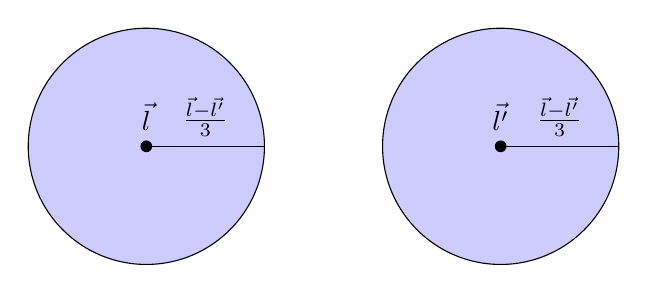
\begin{tikzpicture}[scale=0.75,bullet/.style={circle,fill,inner sep=1.5pt,node contents={}}]
\draw [black,fill=blue!20]  (0,0) circle (2);
\draw [black] (0,0)node[bullet,label=above:$\vec{l}$] --(2,0)node[pos=0.5,above]{ $\frac{\norme{\vec{l}-\vec{l'}}}{3}$ } ;
\draw [black,fill=blue!20]  (6,0) circle (2);
 \draw [black]  (6,0)node[bullet,label=above:$\vec{l'}$] --(8,0)node[pos=0.5,above]{ $\frac{\norme{\vec{l}-\vec{l'}}}{3}$ } ;
\end{tikzpicture}\\
A partir d'un certain rang, tous les termes de la suite doivent appartenir aux deux boules ouvertes ce qui est impossible car l'intersection de ces deux boules est vide
\end{center}
On pose $\epsilon=\frac{\norme{\vec{l}-\vec{l'}}}{3}\overbrace{>}^{\vec{l}\neq \vec{l'}}0$. Comme $(\vec{x_n})_{n\in\N}$ converge vers $\vec{l}$ et $\vec{l'}$, il existe $N$ [resp. $N'$] tel que à partir de ce rang, le termes appartiennent à la boule $B(\vec{l},\frac{\norme{l-l'}}{3})$ [resp. $B(\vec{l'},\frac{\norme{l-l'}}{3})$], c'est à dire,
$$\forall n \geq N:\quad  \norme{\vec{x_n} - \vec{l}} <  \frac{\norme{\vec{l}-\vec{l'}}}{3}$$
et  
$$\forall n \geq N':\quad \norme{\vec{x_n} - \vec{l'}} <  \frac{\norme{\vec{l}-\vec{l'}}}{3}.$$
Soit $N''=\max(N,N')$. On a :
$$\norme{\vec{l} - \vec{l'}}=\norme{(\vec{l} - u_{N''})+ (u_{N''}- \vec{l'})}\leq \norme{\vec{l} - u_{N''}}+ \norme{u_{N''}- \vec{l'}}< \frac{\norme{\vec{l}-\vec{l'}}}{3}+\frac{\norme{\vec{l}-\vec{l'}}}{3}=\frac{2\norme{\vec{l}-\vec{l'}}}{3}.$$ 
Comme $\norme{\vec{l}-\vec{l'}} \neq 0$, on obtient $1< \frac{2}{3}$ ce qui est impossible.
\end{Demonstration}
\begin{Remarque}[Dépendance de la norme en dimension infinie]
La notion de convergence est définie à partir d'une norme. Si on change de norme (et donc on change d'espace vectoriel
normé), il est possible que la suite considérée ne converge plus.\\
En effet, soit la suite $(f_n)_{n\in\N}$ d'éléments $\mathcal{C}([0,1],\K)$ définie par $f_n:x\to x^n.$
On a :
\begin{itemize}
\item $\norme{f_n}_{1}=\int_0^1  |x^n|\,\mathrm{dx}=\frac{1}{n+1}$, donc la suite  $(f_n)_{n\in\N}$ converge vers la fonction nulle dans l'espace vectoriel normé $(\mathcal{C}([0,1],\K), \norme{\,}_{1})$.
\item $\norme{f_n}_{\infty}=\sup_{x\in[0,1]}|x^n|=1$, donc la suite  $(f_n)_{n\in\N}$ ne converge pas vers la fonction nulle dans l'espace vectoriel normé $(\mathcal{C}([0,1],\K), \norme{\,}_{\infty})$.
\end{itemize}
\end{Remarque}
\begin{Proposition}[Bornée si convergente]
Si la suite $(\vec{x_n})_{n\in\N}$ converge pour la norme $\norme{\,}$,\\
Alors la suite $(\vec{x_n})_{n\in\N}$ est bornée pour la même norme $\norme{\,}$.
\end{Proposition}
\begin{Demonstration}
On suppose que $(\vec{x_n})_{n\in\N}$ converge vers $\vec{l}$.\\
En particulier pour $\epsilon=1$, il existe $N\in\N$ tel que :
$$\forall n\geq N:\norme{\vec{x_n}-\vec{l}}<1.$$
 Comme $\norme{\vec{x_n}}-\norme{\vec{l}} \leq \norme{\vec{x_n}-\vec{l}}$, on a 
$$\forall n\geq N:\norme{\vec{x_n}}<1+\norme{\vec{l}}.$$
En posant $M=\max(\norme{\vec{x_0}},\dots,\norme{\vec{x_{N-1}}},1+\norme{\vec{l}} )$, on obtient :
$$\forall n\in N:\norme{\vec{x_n}}<M.$$
Donc $(\vec{x_n})_{n\in\N}$ est bornée.
\end{Demonstration}
\begin{Remarque}
La réciproque de ce proposition est fausse. La suite $((-1)^n)_{n\in\N}$ est bornée mais non convergente.
\end{Remarque}
\begin{Proposition}[Structure d'espace vectoriel]
Soit $(\vec{x_n})_{n\in\N}$ et $(\vec{y_n})_{n\in\N}$ et $\lambda , \mu \in\K$.\\
Si  $(\vec{x_n})_{n\in\N}$ converge vers $\vec{l}$ pour la norme $\norme{\,}$ et  $(\vec{x_n})_{n\in\N}$ converge vers $\vec{l'}$ pour la norme $\norme{\,}$,\\
Alors $(\lambda\vec{x_n}+\mu\vec{y_n} )_{n\in\N}$ converge vers $\lambda\vec{l}+\mu\vec{l'}$  pour la norme $\norme{\,}$.\\
Ainsi, l'ensemble des suites convergentes est un espace vectoriel. 
\end{Proposition}
\begin{Demonstration}
En bref $$\norme{\lambda\vec{x_n}+\mu\vec{y_n}  -\lambda\vec{l}+\mu\vec{l'} } =\norme{\lambda(\vec{x_n}-\vec{l}) +\mu(\vec{y_n}-\vec{l'}) }\leq |\lambda|\norme{\vec{x_n}-\vec{l}} +|\mu|\norme{\vec{y_n}-\vec{l'}}\tend[n\to\infty] 0.$$
\end{Demonstration}
\begin{Proposition}[Suite extraite]
Si $(\vec{x_n})_{n\in\N}$ est une suite convergente vers $\vec{l}$,\\
Alors toute suite extraite $(\vec{x_{\phi(n)}})_{n\in\N}$ converge vers $\vec{l}$. 
\end{Proposition}
\begin{Demonstration}
Soit $\phi$ une fonction strictement croissante de $\N$ dans $\N$.
On suppose $(\vec{x_n})_{n\in\N}$ convergente vers $\vec{l}$.\\
Soit $\epsilon>0$. Il existe $N\in\N$ telle que :
$$\forall n\geq N:\quad \norme{\vec{x_n}-\vec{l}}<\epsilon.$$
Comme $\forall n\in\N: \phi(n)\geq n$, si $n>N$ alors $\phi(n)>N$, donc    
$$\forall n\geq N:\quad \norme{\vec{x_{\phi(n)}}-\vec{l}}<\epsilon.$$
Ainsi, $(\vec{x_{\phi(n)}})_{n\in\N}$ converge vers $\vec{l}$. 
\end{Demonstration}
\subsection{En dimension finie}
\begin{Theoreme}[Indépendance de la norme en dimension finie]
On suppose que $E$ est de dimension finie. Soient $N$ et $N'$ deux normes sur $E$. Soit $(\vec{x_n})_{n\in\N}$ une suite d'éléments de $E$.\\
$(\vec{x_n})_{n\in\N}$ est bornée pour la norme $N$ si et seulement si $(\vec{x_n})_{n\in\N}$ est bornée pour la norme $N'$.\\
$(\vec{x_n})_{n\in\N}$ converge vers $\vec{l}$ pour la norme $N$ si et seulement si $(\vec{x_n})_{n\in\N}$ converge vers $\vec{l}$ pour la norme $N'$.
\end{Theoreme}
\begin{Demonstration}
Comme $E$ un espace vectoriel de dimension finie, il existe deux réels strictement positifs tels que $\alpha N \leq  N'  \leq \beta N$.
\begin{itemize}
\item 
On suppose la suite $(\vec{x_n})_{n\in\N}$
bornée pour la norme $N$. Il existe donc $M \in \R^{+}$ tel que $\forall n\in \N,  N(\vec{x_n})\leq M$. Soit $n\in\N$. On a :
$N'(\vec{x_n})\leq  \beta N(\vec{x_n})\leq \beta M$.
Donc, $(\vec{x_n})_{n\in\N}$
bornée pour la norme $N'$.\\
En permutant les rôles de $N$ et $N'$, on obtient la réciproque.
\item 
On suppose que la suite $(\vec{x_n})_{n\in\N}$ converge vers $\vec{l}$ pour la norme $N$.\\
Soit $\epsilon>0$. Comme  la suite $(\vec{x_n})_{n\in\N}$ converge vers $\vec{l}$ pour la norme $N$, il existe $N\in\N$ tel que
$$\forall n \geq N:\quad  N(\vec{x_n} - \vec{l}) < \frac{\epsilon}{\beta}.$$
Comme $N'(\vec{x_n})\leq  \beta N(\vec{x_n})$, on a 
$$\forall n \geq N:\quad  N'(\vec{x_n} - \vec{l}) < \beta \frac{\epsilon}{\beta}=\epsilon$$
et donc la suite $(\vec{x_n})_{n\in\N}$ converge vers $\vec{l}$ pour la norme $N'$.\\
En permutant les rôles de $N$ et $N'$, on obtient la réciproque.
\end{itemize}
\end{Demonstration}
\begin{Remarque}
Dorénavant, on n'aura donc plus besoin de préciser "pour la norme $N$" lorsqu'on parlera de
convergence, de limite ou de suite bornée dans un espace vectoriel de dimension finie. 
\end{Remarque}
\begin{DefinitionProposition}[Norme infinie attachée à une base en dimension finie]
On suppose que $E$ est de dimension finie muni d'une base $\mathcal{B} = (\vec{e_1}, \dots, \vec{e_p})$.\\
La \defi{norme infinie attachée à la base $\mathcal{B}$}, notée $\norme{\,}_\infty$, est  définie par :
$$\forall \vec{x}=\sum_{i=i}^p x_i\vec{e_i} \in  E:\quad \norme{\vec{x}}_\infty=\max_{1\leq i\leq p}|x_i|.$$ 
\end{DefinitionProposition}
\begin{Demonstration}
Elle est formellement identique à celle qui établit que $\norme{\,}_{\infty}$ est une norme dans $\K^n$.
\end{Demonstration}
\begin{Proposition}[Convergence composante par composante]
On suppose que $E$ est de dimension finie muni d'une base $\mathcal{B} = (\vec{e_1}, \dots, \vec{e_p})$.\\
Soit $(\vec{x_n})_{n\in\N}$ une suite d'éléments de $E$ telle que : 
$$\forall  n\in\N : \quad \vec{x_n} = \sum_{i=1}^p x_{i,n} \vec{e_i}.$$
Alors la suite $(\vec{x_n})_{n\in\N}$ converge dans $E$ si et seulement si les $p$ suites coordonnées $(x_{i,n})_{n\in\N}$ convergent dans $\K$.\\
Dans ce cas, on a $\lim\limits_{n\to\infty} \vec{x_n} = \sum_{i=1}^p (\lim\limits_{n\to\infty}x_{i,n}) \vec{e_i}.$\\
De même pour la notion de bornée.
\end{Proposition}
\begin{Demonstration}
\begin{itemize}
\item $\Longrightarrow$ : On suppose que la suite $(\vec{x_n})_{n\in\N}$ convergeant vers  $\vec{l}=\sum_{i=1}^n l_i \vec{e_i}.$ Comme la notion de convergence ne dépend pas la norme, on choisit la convergence suivant la norme $\norme{\,}_\infty$ dans la base $\mathcal{B}$. On a alors :
$$\forall \epsilon >0,\exists N\in \N, \forall n\geq N:\quad \norme{\vec{x_n}-\vec{l}}=\max_{1 \leq i \leq p }|x_{i,n}-l_i|<\epsilon \text{ et donc }\forall i\in\Intf{1}{p}|x_{i,n}|<\epsilon.$$
Donc toutes les suites $(x_{i,n})_{n\in\N}$ convergent respectivement vers $l_i$.
\item $\Longleftarrow$ : On suppose les suites $(x_{i,n})_{n\in\N}$ convergent respectivement vers $l_i$. On a :
$$\forall \epsilon >0, \forall i\in\Intf{1}{p},\exists N_i\in \N, \forall n\geq N_i:\quad |x_{n,i}-l_i|<\epsilon.$$
En posant $N_m=\max(N_1,\dots,N_p)$, on a   $\forall i\in\Intf{1}{p}, \forall n\geq N:\quad |x_{n,i}-l_i|<\epsilon$, donc $\norme{\vec{x_n}-\vec{l}}=\max_{1 \leq i \leq p }|x_{i,n}-l_i|<\epsilon$ avec $\vec{l}=\sum_{i=1}^n l_i \vec{e_i}$.
\end{itemize}
\end{Demonstration}
\begin{Exemple}[Convergence de matrices]
La suite de matrices $\left(\begin{pmatrix}
\frac{\ln(n)}{n}& (1+\frac{1}{n})^n\\ \sum_{k=1}^{n}\frac{1}{k^2}&0
\end{pmatrix}\right)_{n\in\N}$ converge et a pour limite $\begin{pmatrix}
0& e\\ \frac{\pi^2}{6}&0
\end{pmatrix}$ car $\lim\limits_{n\to\infty}\frac{\ln(n)}{n}=0$, $\lim\limits_{n\to\infty}(1+\frac{1}{n})^n=e$ et $\sum_{k=1}^{\infty}\frac{1}{k^2}=\frac{\pi^2}{6}$.
\end{Exemple}

%
%% -----------------------------------------------------------------------------
\section{Topologie d'un espace vectoriel normé de dimension finie}
Un espace vectoriel $E$ de dimension finie peut toujours être identifié à $\K^n$ en identifiant les coordonnées d'un vecteur dans une base de $E$ et les coordonnées dans la base canonique de $\K^n$. Tous les énoncés ci-dessous concernant $\K^n$ s'étendent donc à un tel $E$ muni de la topologie transportée par cette identification. On ne précisera pas "pour la norme $N$" car  la topologie de $\K^n$ ne dépend pas du choix de la norme sur $\K^n$. 

\subsection{Point intérieur, point adhérent}
Un point est à l'intérieur d'une partie $A$ si tous les points autour de celui-ci sont encore dans $A$ à condition de ne pas trop s'éloigner.
\begin{Definition}[Intérieur]
Soit $A$ une partie de $\K^n$.\\
$\vec{x}$ est \defi{intérieur} à $A$ si $$\exists  r > 0, B (\vec{x}, r) \subset A.$$
L'\defi{intérieur de $A$}, notée $\stackrel {\ \circ }{A}$, est l'ensemble des points intérieurs à $A$.\\
%$\stackrel {\ \circ }{A}$ est le plus grand (au sens de l'inclusion) ouvert de $E$ contenu dans $A$.
\end{Definition}
\begin{Exemple}
L'intérieur de $[0,1[$ est $]0,1[$.\\
L'intérieur de  $A  =\Big\{(x,y)\in\R^2\ |\ 0\leq x<5 \Big\}$ est  
$A  =\Big\{(x,y)\in\R^2\ |\ 0< x<5 \Big\}$.\\
L'intérieur de $\Q$ dans $\R$ est $\emptyset$ car  toute boule ouverte de $\R$ centrée sur un rationnel contient au moins un irrationnel.
\end{Exemple}
\begin{Definition}[Adhérent]
Soit $A$ une partie de $\K^n$.\\
$\vec{x}$ est \defi{adhérent} à $A$ si $$\forall  r > 0, B (\vec{x}, r) \cap A\neq \emptyset .$$
L'\defi{adhérence de $A$}, notée $\overline {A}$, est l'ensemble des points adhérents à $A$.\\
%$\overline {A}$ est le plus petit (au sens de l'inclusion) fermé de $\K^n$ contenant  $A$.
\end{Definition}
\begin{Exemple}
L'adhérence de de $]0,1[$ est $[0,1]$.\\
L'adhérence de  $A  =\Big\{(x,y)\in\R^2\ |\ 0\leq x<5 \Big\}$ est  
$A  =\Big\{(x,y)\in\R^2\ |\ 0\leq x\leq5 \Big\}$.\\
L'adhérence de $\Q$ dans $\R$ est $\R$ car  toute boule ouverte de $\R$ contient au moins un rationnel.
\end{Exemple}
\begin{Proposition}
Soit $A$ une partie de $\K^n$.\\
$\vec{x}$ est adhérent à $A$ si et seulement si il existe une suite $(\vec{x_n})_{n\in\N}$
d'éléments de $A$, convergente, de limite $\vec{x}$.
\end{Proposition}
\begin{Demonstration}
\begin{itemize}
\item $\Rightarrow :$ Soit $\vec{x}$ un point adhérent. On peut donc construire la suite $(\vec{x_n})_{n\in\N}$ tel que $\vec{x_n}\in B (\vec{x}, \frac{1}{n+1} )$. Cette suite converge vers $\vec{x}$. 
\item $\Leftarrow :$ Soit une suite $(\vec{x_n})_{n\in\N}$ d'éléments de $A$, convergente, de limite $\vec{x}$. Donc, quelque soit $r>0$, à partir d'un certain rang, tous le termes de la suite appartiennent à  $B (\vec{x}, r)$, donc $B (\vec{x}, r) \cap A\neq \emptyset$ car $(\vec{x_n})_{n\in\N}$ est une suite d'éléments de $A$.
\end{itemize}
\end{Demonstration}
Une partie dense est une partie permettant d'approcher tous les éléments de l'espace englobant.
\begin{Definition}[Dense]
$A$ est \defi{dense} dans $\K^n$ si $\overline {A}=\K^n$
\end{Definition}
\begin{Exemple}
$\Q$ est dense dans $\R$.
\end{Exemple}
\begin{Definition}[Frontière]
La \defi{frontière} de $A$ est $\overline {A}\setminus \stackrel {\ \circ }{A}.$
\end{Definition}
\begin{Exemple}
La frontière de $[0,1[$ est $ \{0,1\}$.\\
La frontière  de  $A  =\Big\{(x,y)\in\R^2\ |\ 0\leq x<5 \Big\}$ est  
$A  =\Big\{(x,y)\in\R^2\ |\ x=0\text{ ou } x=5  \Big\}$.\\ 
La frontière  $\Q$ dans $\R$ est $\R$.
\end{Exemple}

\subsection{Ouverts et fermés}

Un ouvert $A$ est une partie de $E$ qui présente la propriété caractéristique suivante : en choisissant comme origine un point quelconque de ce sous-ensemble, tous les points autour de celui-ci sont encore dans $A$ à condition de ne pas trop s'éloigner. C'est à dire si tous ses points sont à l'intérieur de lui-même. 
\begin{Definition}[Ouvert et fermé]
\begin{itemize}
\item Une \defi{partie ouverte} de $\K^n$, ou plus simplement un \defi{ouvert} de $\K^n$, est une partie $A$ de $\K^n$ telle que $$\forall \vec{x}\in A, \exists r>0:\quad B(\vec{x},r)\subset \K^n$$
c'est à dire  $\stackrel {\ \circ }{A}=A.$
\item Une \defi{partie fermée} de $\K^n$, ou plus simplement un \defi{fermé} de $\K^n$, est une partie $F$ de $\K^n$ telle que le complémentaire de $\K^n$ dans $F$, $\K^n\setminus F$, est un ouvert de $\K^n$.
\end{itemize}
Par convention, l'ensemble vide $\emptyset$ et $\K^n$ sont à la fois ouverts et fermées dans $\K^n$.
\end{Definition}
%\begin{Exemple}
%L'ensemble $]0,1[$ est un ouvert de $\R$.
%\end{Exemple}
\begin{Proposition}[Boule ouverte]
\begin{itemize}
\item La boule ouverte est une partie ouverte de $\K^n$.
\item La boule fermée  est une partie fermée de $\K^n$.
\end{itemize}
\end{Proposition}
\begin{Demonstration}$,$\\
\begin{minipage}[c]{0.6\linewidth}{
Soit $B(\vec{x},r)$ une boule ouverte.\\
Soit $\vec{x'}\in B(\vec{x},r)$. \\
On choisit un $r'$ tel que $0< r' < r -\norme{\vec{x}-\vec{x'}}$.\\
Soit $\vec{y}\in B(\vec{x'},r')$. On a $\norme{\vec{x}-\vec{y}}=\norme{(\vec{x}-\vec{x'})+(\vec{x'}-\vec{y})}\leq \norme{\vec{x}-\vec{x'}} + \norme{\vec{x'}-\vec{y}}<r.$ Donc $B(\vec{x'},r')\subset B(\vec{x},r).$
}
\end{minipage} 
    \begin{minipage}[c]{0.4\linewidth}{\hspace*{0.2\linewidth}
    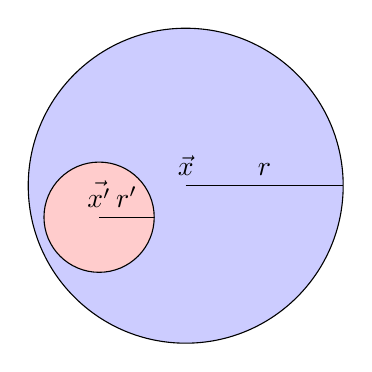
\begin{tikzpicture}
\draw [black,fill=blue!20]  (0,0) circle (2);
\draw [black] (0,0)node[above]{ $\vec{x}$ } --(0:2)node[pos=0.5,above]{ $r$ };
\draw [black,fill=red!20]  (-1.1,-0.4) circle (0.7);
\draw [black] (-1.1,-0.4)node[above]{ $\vec{x'}$ } --(-0.4,-0.4)node[pos=0.5,above]{ $r'$ };
\end{tikzpicture}\begin{tiny}
%Identification coordonnées d'un vecteur avec coordonnées d'un point
\end{tiny}
}
\end{minipage} 
\end{Demonstration}
\begin{Exemple}[Intervalle ouvert]
Un intervalle ouvert $]a,b[$ de $\R$ est un ouvert de $\R$ car $]a,b[=B(\frac{a+b}{2},\frac{b-a}{2})$.
\end{Exemple}
\begin{Exemple}[Singleton fermé]
\begin{minipage}[c]{0.6\linewidth}{
Les singletons sont des fermés.\\ 
Soit $\vec{x}\in \K^n$.\\
Soit $\vec{y}\in K^n\setminus \{\vec{x}\}$. On pose $r=\frac{\norme{\vec{x}-\vec{y}}}{2}$.
$\vec{x}\notin B(\vec{y},r)$ car $\norme{\vec{x}-\vec{y}}\geq r$. On a $B(\vec{y},r)\subset K^n\setminus \{\vec{x}\}$.\\
Ainsi $K^n\setminus \{\vec{x}\}$ est un ouvert donc  $\{\vec{x}\}$ est un fermé.
}
\end{minipage} 
    \begin{minipage}[c]{0.4\linewidth}{\hspace*{0.2\linewidth}
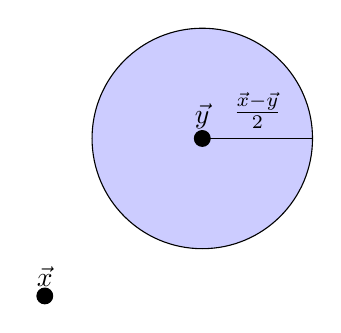
\begin{tikzpicture}[scale=2] 
\draw [fill=black]  (0,0)node[above]{ $\vec{x}$ } circle (0.05);
\draw [black,fill=blue!20]  (1,1) circle (0.7);
\draw [black] (1,1) --(1.7,1)node[pos=0.5,above]{ $\frac{\norme{\vec{x}-\vec{y}}}{2}$ } ;
\draw [fill=black]  (1,1)node[above]{ $\vec{y}$ } circle (0.05);
\end{tikzpicture}\\\begin{tiny}
%Identification coordonnées d'un vecteur avec coordonnées d'un point
\end{tiny}
}
\end{minipage} 
\end{Exemple}
\begin{Proposition}[Propriétés des ouverts]
\begin{itemize}
\item $\emptyset$ et $\K^n$ sont des ouverts et des fermés.
\item \emph{stabilité par union quelconque}:
  Si $\forall i\in I$, $U_i$ est un ouvert de $\K^n$, alors $\cup_{i\in I} U_i$ est un ouvert de $\K^n$.
\item \emph{stabilité par intersection finie}:
  Si $U_1, \dots, U_n$ sont des ouverts de $\K^n$, alors $\cap_{i=1}^n U_i$ est un ouvert de $\K^n$.
\end{itemize}
\end{Proposition}
\begin{Demonstration}
\begin{itemize}
\item \emph{stabilité par union quelconque}:
  Soit $(U_i)_{i\in I}$ une famille d'ouverts de $\K^n$.\\
  Soit $\vec{x}\in\cup_{i\in I} U_i$. Il existe un indice $i\in I$ tel que $\vec{x}\in U_i$.\\
  Comme $U_i$ est un ouvert, il existe $r>$ tel que $B(\vec{x},r)\subset U_i$.\\
  Comme  $U_i\subset \cup_{j\in I} U_j$, $B(\vec{x},r)\subset\cup_{j\in I} U_j$.
\item \emph{stabilité par intersection finie}:
  Soit $(U_i)_{1\leq i\leq n}$ une famille finie d'ouverts de $\K^n$.\\
 Soit $\vec{x}\in\cap_{i\in I} U_i$. Pour tout indice $i\in \Intf{1}{n}$, $\vec{x}\in U_i$.\\
  Comme $U_i$ est un ouvert, il existe $r_i>$ tel que $B(\vec{x},r_i)\subset U_i$.\\
  Soit $r=\min(r_1,\dots,r_n)$. Donc, pour tout indice $i\in \Intf{1}{n}$, $B(\vec{x},r)\subset B(\vec{x},r_i)\subset U_i$.\\
  Ainsi $B(\vec{x},r)\subset \cap_{i=1}^n U_i$ et $\cap_{i=1}^n U_i$ est un ouvert. 
\end{itemize}
\end{Demonstration}
\begin{Remarque} La propriété de stabilité par une intersection non finie est fausse.\\
Considérons la famille dénombrable d'ouverts $(A_n)_{n\in\N^*}$ définie par : $A_n =]-\frac 1 n ,\frac 1 n[$. 
Il est ici tout à fait évident que $(A_n)_{n\in\N^*}$ est une famille d'ouvert. On a :
$$\cap_{n\in\N^*}]-\frac 1 n ,\frac 1 n[=\{0\}.$$
Le singleton $\{0\}$ n'est pas un ouvert ce qui montre que l'intersection dénombrable d'une famille d'ouverts n'est
pas nécessairement un ouvert.
\end{Remarque}
\begin{Exemple}[Dans $\R$]
$]0,+\infty[$ est un ouvert car union d'ouverts $\cup_{n\in \N^*}]0,n[$ et et plus généralement les intervalles de la forme $]a,+\infty[$ ou $]-\infty,a[$ sont des ouvert de $\R$.
\end{Exemple}


\begin{Theoreme}[Caractérisation séquentielle des fermés]
Soit $F$ une partie non vide de $\K^n$.\\
F est fermée si et seulement si pour toute suite convergente $(\vec{x_n})_{n\in\N}$
d'éléments de F, la limite, $\lim\limits_{n\to\infty}\vec{x_n}$,  est un élément de $F$.
\end{Theoreme}
\begin{Demonstration}
Soit $F$  une partie non vide de $\K^n$.\\
\begin{itemize}
\item $\Longrightarrow$ :   Soit $F$ est un fermé  de $\K^n$. Soit $(\vec{x_n})_{n\in\N}$ une suite d'éléments de $F$  convergeant vers $\vec{l}$.
Supposons par l'absurde que $\vec{l}\notin F$, c'est à dire que    $\vec{l}$ appartient au complémentaire du fermé $F$, $\K^n\setminus F$, qui est donc ouvert. Il existe alors une boule ouverte $B$ de centre $\vec{l}$  et de rayon $r > 0$ inclue dans $\K^n\setminus F$.  Aucun élément de la suite appartient à cette boule.\\ 
Comme la suite converge vers  $\vec{l}$, à partir d'un certain rang, tous les termes de la suite appartiennent à cette boule ouverte.\\
 D'où la contradiction. 
\item  $\Longleftarrow$ : par contreproposition, soit $F$ une partie non fermé de $\K^n$. Donc la complémentaire de $F$, $\K^n\setminus F$, n'est par un ouvert. Il existe alors un élément $\vec{l}$ de $\K^n\setminus F$ telle que toute boule ouverte de centre $\vec{l}$ contient un élément qui n'est pas dans $\K^n\setminus F$ et qui est donc dans $F$. En particulier, on peut construire une suite $(\vec{x_n})_{n\in\N}$ d'éléments de $F$  tel que $\vec{x_n}\in B(\vec{l},\frac 1 n )$. 
Cette suite $(\vec{x_n})_{n\in\N}$ d'éléments de $F$ converge vers $\vec{l}\notin F$.
\end{itemize}
\end{Demonstration}
\begin{Exemple}
$A=\{(x,y)\in \R^2:xy=1\}$ est un fermé.\\
Soit $(x_n,y_n)_{n\in\N}$ une suite d'éléments de $A$ qui converge vers $(x,y)\in \R^2$. Les deux suites coordonnées $(x_n)_{n\in\N}$ et $(y_n)_{n\in\N}$ convergent vers $x$ et $y$ respectivement. Pour tout $n \in \N: x_ny_n=1$, par passage à la limite, on a : $\lim\limits_{n\to\infty}(x_ny_n)=\lim\limits_{n\to\infty}(1)=1$. Comme les deux suites coordonnées convergent, 
 $\lim\limits_{n\to\infty}(x_ny_n)=\lim\limits_{n\to\infty}x_n\lim\limits_{n\to\infty}y_n=xy=1$. Ainsi la limite appartient à $A$.
D'après la caractérisation séquentielle des fermé, A est fermé.
\end{Exemple}
\begin{Exemple}[Matrice symétrique]
L'ensemble des matrices symétriques $\SnR=\{M\in\Mn{n}{\R}:\transposee{M=M}\}$ est un fermé.\\
Soit $(S_p=(s^p_{i j})_{1\leq i,j\leq n} )_{p\in\N}$ une suite d'éléments de $\SnR$ qui converge vers $M=(m_{ij})_{1\leq i,j\leq n}\in \Mn{n}{\R}$.\\
Comme $S_n$ est symétrique, $s^p_{i j}=s^p_{j i}$. Comme les suite coordonnées convergent, par passage à la limite on a $m_{ij}=\lim\limits_{p\to\infty}(s^p_{i j})=\lim\limits_{p\to\infty}(s^p_{j i})=m_{ji}$. Ainsi $M$ est symétrique.\\ 
D'après la caractérisation séquentielle des fermé, $\SnR$ est fermé.
\end{Exemple}
\begin{Definition}[Bornée et compact]
Une partie $A$ de $\K^n$ est dite \defi{bornée} s'il existe une boule ouvert $B$ qui le contient.\\
Il est dit \defi{compact} si cette partie est fermée et bornée. 
\end{Definition}
\begin{Exemple}
Les droites, demi-droites et demi-plans sont fermées non bornées dans le plan $\R^2$ ou dans l'espace $\R^3$. De même, les plans sont fermés non bornés dans $\R^3$.\\
Toute boule ouverte de $\R^n$ est ouverte et bornée. Toute boule fermée est compacte.\\
L'ensemble $A=\{(x,y)\in\R^2: 0\leq x \leq 1\text{ et }0\leq y\leq x^2\}$ est un compact.\\
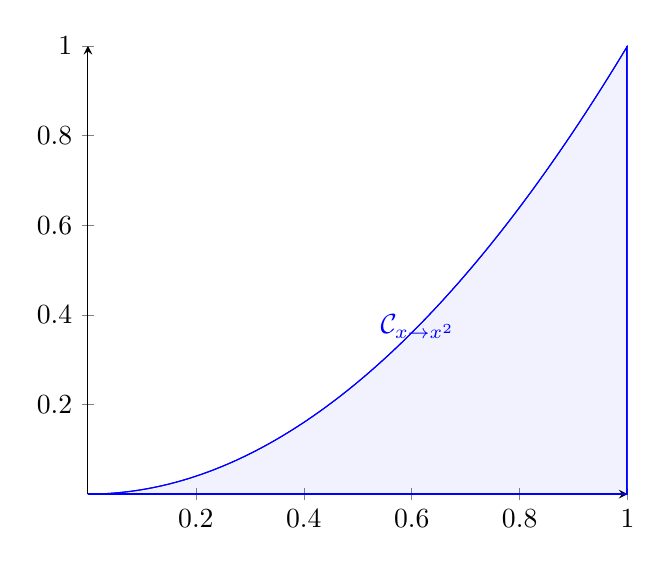
\begin{tikzpicture}
   \begin{axis}[
       axis y line = middle,
       axis x line = middle,
       samples     = 200,
       domain      = 0:1,
       xmin = 0, xmax = 1,
       ymin = 0, ymax = 1,
       unbounded coords=jump
     ]
     \addplot[domain=0:1,blue] {x^2}node[pos=0.5] {$\mathcal{C}_{x\to x^2}$};
         \addplot[domain=-0:1,blue,fill=blue, 
                    fill opacity=0.05] {x^2}\closedcycle ;
        \addplot [thick,color=blue]coordinates {
            (1, 1) 
            (1, 0)
            (0, 0)  }; 
   \end{axis}

\end{tikzpicture}

\end{Exemple}
\begin{Theoreme}[Bolzano-Weierstrass]
Une partie $A$ de $\K^n$ est compact  si et seulement si toute suite d'éléments de $A$ admet une sous-suite qui converge vers un élément de X.
\end{Theoreme}
\begin{Exemple}
La suite $(\sin n)_{n\in\N}$ est à valeurs dans le compact $[-1,1]$. Donc il existe une sous-suite convergente.\\
Un résultat plus fort faisant appel à la théorie des groupes est que pour toute valeur de $[-1,1]$, il existe une sous-suite convergeant vers cette valeur.   
\end{Exemple}

\section{Étude locale d'une application - continuité}
\subsection{Limite}
%\begin{minipage}[c]{0.45\linewidth}{
De manière intuitive, une fonction admet pour limite $\vec{l}$ en $\vec{a}$ quand $f(\vec{x})$ se rapproche  de $\vec{l}$,  quand  la variable $\vec{x}$ se rapproche de $\vec{a}$. Une définition plus rigoureuse est 
\begin{itemize}  
\item "$f(\vec{x})$ se rapproche de $\vec{l}$"; pour tout rayon $\epsilon$, $f(\vec{x})$ appartient à la boule centrée en $\vec{l}$ et de rayon $\epsilon$
\item  "la variable $\vec{x}$ se rapproche de $\vec{a}$" : il existe un rayon $\delta$ telle cette propriété est vraie pour tous $\vec{x}$ appartenant à la boule centrée en $\vec{a}$ et de rayon $\delta$. 
\end{itemize} 
%}
%\end{minipage} \hfill
%    \begin{minipage}[r]{0.5\linewidth}{
%\hspace*{0.1\linewidth}
\begin{center} 
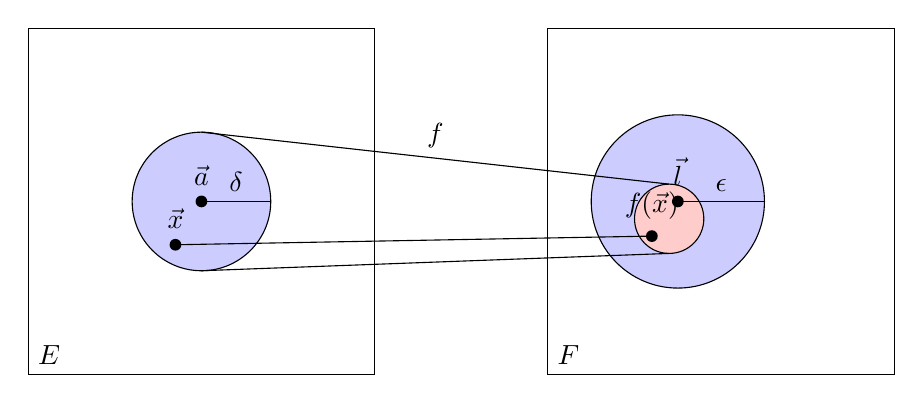
\begin{tikzpicture}[scale=1.1,bullet/.style={circle,fill,inner sep=1.5pt,node contents={}}]
\draw (-5,0) rectangle (-1,4) node[above right] at (-5,0) {$E$};
\draw (1,0) rectangle (5,4)node[above right] at (1,0) {$F$};

\draw [black,fill=blue!20]  (-3,2) circle (0.8);
\draw [black,fill=blue!20]  (2.5,2) circle (1);
\draw [black,fill=red!20]  (2.4,1.8) circle (0.4);
\draw (-3.3,1.5)node[bullet,label=above:$\vec{x}$] --(2.2,1.6)node[bullet,label=above:$f(\vec{x})$] ; 

\draw (-3,2)node[bullet,label=above:$\vec{a}$] --(-2.2,2)node[pos=0.5,above]{ $\delta$} ; 
\draw (2.5,2)node[bullet,label=above:$\vec{l}$] --(3.5,2)node[pos=0.5,above]{ $\epsilon$} ; 


\draw (-3,2.8) -- (2.4,2.2)node[pos=0.5,above]{ $f$};
\draw (-3,1.2) -- (2.4,1.4);
\end{tikzpicture}\\
 Exemple d'une application de $f:E\to F$. Quelque soit le rayon $\epsilon$, il existe un rayon $\delta$, telle que $f(B(\vec{a},\delta))\subset B(\vec{l},\epsilon)$.
 \end{center}
%}
%\end{minipage} 
\begin{Definition}[Limite]
Soit $A$ une partie non vide de $E$, $\vec{a}$ un point de $E$ adhérent à $A$, $f : A \to F$ et $\vec{l} \in F$.\\
$f$ admet $\vec{l}$ pour \defi{limite} au point $\vec{a}$ si
$$\forall \epsilon >0,  \exists \delta > 0,   \overbrace{\forall \vec{x} \in A: \quad  \norme{\vec{x} - \vec{a}}_E < \delta}^{\vec{x}\in B(\vec{a},\delta)\cap A}   \Rightarrow \overbrace{\norme{f (\vec{x}) - \vec{l}} < \epsilon.}^{f(\vec{x})\in B(\vec{l},\epsilon)}$$
Lorsqu'un tel $\vec{l}$ existe il est unique ; on dit alors que $\vec{l}$ est \defi{la limite de $f$ en $\vec{a}$} et l'on note :
$$\lim_{\vec{x}\to\vec{a} } f(\vec{x})= \vec{l}.$$
\end{Definition}
\begin{Exemple}
Soit $\Fonction{f}{\R\setminus \{0\}}{\R}{x}{\frac{\sin x }{x}} $.\\
 $0$ est adhérent à $\R\setminus \{0\}$ et la fonction admet $1$ pour limite en $0$ du fait du développement limité à l'ordre 1 en 0 de la fonction sinus ($\sin x = x + o(x)$, d'où $\frac{\sin x}{x} = 1 + o(1)$).
\end{Exemple}
%TODO AUTRE Exemple par exemple racine(x) limite en 0

%\begin{Exemple}
%Soit $\Fonction{f}{\R\setminus \{0\}}{\R}{x}{\frac{\sin x }{x}} $.\\
% $0$ est adhérent à $\R\setminus \{0\}$ et la fonction admet $1$ pour limite en $0$.   
%\end{Exemple}

\begin{Theoreme}[Caractérisation séquentielle]
Une fonction $f$ admet $\vec{l}$ pour limite au point $\vec{a}$ si et seulement si, pour tout suite $(\vec{x_n})_{n\in\N}$  telle que $\lim\limits_{n\to\infty}\vec{x_n}=\vec{a}$ alors $\lim\limits_{n\to\infty}f(\vec{x_n})=\vec{l}$.
\end{Theoreme}
\begin{Remarque}
Ce théorème permet de lier la notion de limite de fonction à celle de limite d'une suite.\\
Cette caractérisation peut surtout être utile pour prouver qu'une fonction n'admet pas de limite. \\
Soit $\Fonction{f}{\R^2\setminus \{(0,0)\}}{\R}{(x,y)}{\frac{x y }{x^2+y^2}} $.\\
Soit $u_n=(\frac 1 n,0)$ et $v_n=(\frac 1 n,\frac 1 n)$. 
On a $\lim\limits_{n\to\infty}u_n=\lim\limits_{n\to\infty}v_n=(0,0)$ mais $\lim\limits_{n\to\infty}f(u_n)=\lim\limits_{n\to\infty}0=0$ et $\lim\limits_{n\to\infty}f(v_n)=\lim\limits_{n\to\infty}\frac{1}{2}=\frac{1}{2}.$ Donc $f$ n'admet pas de limite en $(0,0)$.
\end{Remarque}
\begin{Proposition}[Limite composante par composante]
Soit $E$ et $F$ deux espaces vectoriels normés avec $F$ de dimension finie munie d'une base $\mathcal{B}=(\vec{e_1},\dots, \vec{e_p})$.\\
Soit $f:A\to F$ avec $A\subset E$. Soit $\vec{a}$ un point adhérent à $A$.
On note  $(f_1, \dots, f_p)$ les fonctions composantes de $f $dans la base
$\mathcal{B}$, c'est-à-dire : $$f=f_1\vec{e_1}+\dots + f_p\vec{e_p}.$$
$f$ admet une limite en $\vec{a}$ si et seulement si les fonctions composantes $(f_1, \dots, f_p)$ admettent des limites en $\vec{a}$.\\
Dans ce cas, $$\lim_{\vec{x}\to\vec{a} } f(\vec{x})= \lim_{\vec{x}\to\vec{a} } f_1(\vec{x})\vec{e_1}+\dots+\lim_{\vec{x}\to\vec{a} } f_p(\vec{x})\vec{e_p}.$$
\end{Proposition}
\subsection{Continuité}

En mathématiques, une fonction continue est une fonction qui n'a pas de changements brusques de valeur, appelés discontinuités. Pour une fonction de variable réelle, ces discontinuités sont la nécessité de lever le crayon pour tracer le graphe en ces points. La discontinuité donc la continuité est une \impo{propriété locale} de la fonction.\\
En première approche, une définition rigoureuse de la continuité est donnée en termes d'idée de limite. Une fonction $f$ de la variable $\vec{x}$ est dite continue au point $\vec{a}$ , si la limite de $f(\vec{x})$, lorsque $\vec{x}$ s'approche de ce point $\vec{a}$, est égale à la valeur $f(\vec{a})$; et deuxièmement, la fonction (dans son ensemble) est dite continue sur $A$, si elle est continue en tout point de $A$.

\begin{Definition}[Continuité]
Soit $E$ et $F$ deux espaces vectoriels normés et $A\subset E$.\\
Soit $f:A\to F$.\\
On dit que $f$ est \defi{continue en $\vec{a}\in A$} si $\lim\limits_{\vec{x}\to\vec{a} } f(\vec{x})= f(\vec{a})$.\\
On dit que $f$ est \defi{continue} si elle est continue en tout point de $A$.
\end{Definition}
\begin{Proposition}[Opérations sur les fonctions continues]
Soit $E$, $F$ et $G$ trois espaces vectoriels normés et $A\subset E, B\subset F$.
\begin{itemize}
\item \textit{Combinaison linéaire} :  soit $f:A\to F$ et $g:A\to F$ et $\lambda,\mu\in\K$.\\
Si $f$ et $g$ sont continues en $\vec{a}\in A$ (ou continues sur $A$),\\
Alors $\lambda.f + \mu.g$ est continue en $\vec{a}$ (ou sur $A$).
\item\textit{Multiplication} :  soit $f:A\to F$ et $g:A\to F$.\\
Si $f$ et $g$ sont continues en $\vec{a}\in A$ (ou continues sur $A$),\\
Alors $f \times g$ est continue en $\vec{a}$ (ou sur $A$).
\item\textit{Division} :  soit $f:A\to F$ et $g:A\to F$.\\
Si $f$ et $g$ sont continues en $\vec{a}\in A$ (ou continues sur $A$) et $g$ ne s'annule pas en $\vec{a}$,\\
Alors $\frac{f}{g}$ est continue en $\vec{a}$ (ou sur $A$).
\item\textit{Composition} :  soit $f:A\to B$, $g:B\to G$.\\
Si $f$ est continues en $\vec{a}\in A$ et $g$ est continue en $f(\vec{a})$,\\
Alors $g\circ f$ est continue en $\vec{a}$.
\end{itemize}
\end{Proposition}
\begin{Proposition}[Continuité et coordonnées]
Soit $E$ et $F$ deux espaces vectoriels normés avec $F$ de dimension finie avec $\mathcal{B}=(\vec{e_1},\dots, \vec{e_p})$ une base de $F$.\\
Soit $f:A\to F$ avec $A\subset E$.
On note  $(f_1, \dots, f_p)$ les fonctions composantes de $f $dans la base
$\mathcal{B}$, c'est-à-dire : $$f=f_1\vec{e_1}+\dots + f_p\vec{e_p}.$$
$f$ est continue en $\vec{a}\in A$ si et seulement si les fonctions $(f_1, \dots, f_p)$ sont toutes continues en $\vec{a}\in A$.
\end{Proposition}
\begin{Exemple}[Transposée]
L'application transposée $\transposee{}:\begin{pmatrix}a_{1,1}&a_{1,2}&\cdots &a_{1,p}\\a_{2,1}&a_{2,2}&\cdots &a_{2,p}\\\vdots &\vdots &\ddots &\vdots \\a_{n,1}&a_{n,2}&\cdots &a_{n,p}\\\end{pmatrix} \mapsto\begin{pmatrix}a_{1,1}&a_{2,1}&\cdots &a_{n,1}\\a_{1,2}&a_{2,2}&\cdots &a_{n,2}\\\vdots &\vdots &\ddots &\vdots \\a_{1,p}&a_{2,p}&\cdots &a_{n,p}\\\end{pmatrix}$ est continue car les fonctions coordonnées $\transposee{}_{i j}:\begin{pmatrix}a_{1,1}&a_{1,2}&\cdots &a_{1,n}\\a_{2,1}&a_{2,2}&\cdots &a_{2,n}\\\vdots &\vdots &\ddots &\vdots \\a_{n,1}&a_{n,2}&\cdots &a_{n,n}\\\end{pmatrix}\mapsto a_{j i}$ sont continues.
\end{Exemple}


\begin{Exemple}[Fonction polynomiale]
\begin{itemize}
\item La fonction $f:(x,y)\mapsto xy$ est continue sur $\R^2$ car $p_1:(x,y)\mapsto x $ et $p_2:(x,y)\mapsto y $ sont continues et $f$ est le produit de $p_1$ et $p_2$ ($f(x,y)=(p_1\times p_2)(x,y)=p_1(x,y)\times p_2(x,y) = x y$). 
\item La fonction polynôme à plusieurs variables $P:(x_1,\dots,x_n)\mapsto \sum\limits_{k_{1},\ldots ,k_{n}\in \{0,\ldots ,d_{j}\}}a_{k_{1},\ldots ,k_{n},j}x_{1}^{k_{1}}\ldots x_{n}^{k_{n}}$ est continues comme somme de produits de fonctions continues. 
\end{itemize}
Applications :
\begin{itemize}
\item La fonction déterminant $\Det[]:M \mapsto \Det[] M $ est continue car le déterminant est polynomial en les coordonnées.
\item La fonction polynôme caractéristique $\chi:M \mapsto \Det[](XI_n-M) $ est continue comme composée de fonctions continues $g:M\mapsto XI_n-M$ et de fonction déterminant. La fonction $$g:\begin{pmatrix}a_{1,1}&a_{1,2}&\cdots &a_{1,n}\\a_{2,1}&a_{2,2}&\cdots &a_{2,n}\\\vdots &\vdots &\ddots &\vdots \\a_{n,1}&a_{n,2}&\cdots &a_{n,n}\\\end{pmatrix} \mapsto \begin{pmatrix}X-a_{1,1}&a_{1,2}&\cdots &a_{1,n}\\a_{2,1}&X-a_{2,2}&\cdots &a_{2,n}\\\vdots &\vdots &\ddots &\vdots \\a_{n,1}&a_{n,2}&\cdots &X-a_{n,n}\\\end{pmatrix}$$ est continue car les fonctions coordonnées $g_{i j}:\begin{pmatrix}a_{1,1}&a_{1,2}&\cdots &a_{1,n}\\a_{2,1}&a_{2,2}&\cdots &a_{2,n}\\\vdots &\vdots &\ddots &\vdots \\a_{n,1}&a_{n,2}&\cdots &a_{n,n}\\\end{pmatrix}\mapsto X\delta_{i,j}-a_{i j}$ sont continues.
\end{itemize}
\end{Exemple}

\begin{DefinitionProposition}[Prolongement par continuité]
Soit $E$ et $F$ deux espaces vectoriels normés et $A\subset E$. Soit $\vec{a}\in E$ un point adhérent à $A$ n'appartenant pas à $A$.\\
Soit $f:A\to F$ continue sur $A$ et $f$ admet une limite $\vec{l}$ en $\vec{a}$.\\
Alors le \defi{prolongement par continuité} de $f$  en $\vec{a}$ est la fonction $g$ définie sur $A\cup\{\vec{a}\}$ par
$$\Fonction{g}{A\cup\{\vec{a}\}}{F}{\vec{x}}{\begin{cases}f(\vec{x}),&{\mbox{si }}\vec{x}\neq \vec{a}\\\vec{l} ,&{\mbox{si }}\vec{x}=\vec{a}.\end{cases}}$$
\end{DefinitionProposition}
\begin{Exemple}
La fonction $x\mapsto \frac{\sin x}{x}$ est continue sur $\R\setminus \{0\}$ et admet une limite en 0. Donc elle est prolongeable par continuité en 0.
\end{Exemple}
\subsection{Fonctions lipschitziennes}
Une fonction lipschitzienne est une application possédant une certaine propriété de régularité qui est plus forte que la continuité. Intuitivement, c'est une fonction qui est limitée dans sa manière d'évoluer
\begin{Definition}[Fonctions lipschitziennes]
Soit $(E,\norme{}_E)$ et $(F,\norme{}_F)$ deux espaces vectoriels normés et $A\subset E$. Soit $f:A\to F$.Soit $k>0$. L'application $f$ est dite \defi{$k$-lipschitzienne} si 
$$\forall x,y\in A,\quad\norme{f(x)-f(y)}_F\leq k \norme{x-y}_E.$$
L'application $f$ est dite \defi{lipschitzienne} si il existe $k>0$ telle que $f$ soit $k$-lipschitzienne.
\end{Definition}
\begin{Proposition}[Continuité des fonctions lipschitziennes]
Soit $f:A\to F$ une fonction lipschitzienne.\\
Alors $f$ est continue. 
\end{Proposition}
\begin{Demonstration}
Soit $k>0$ tel que $f$ est $k$-lipschitzienne.\\
Soit $ \vec{a} \in E$ et soit $\epsilon > 0$.
On pose $\delta=\frac{\epsilon}{k}$.\\
Soit $\vec{x}\in E$ tel que  $\norme{\vec{x}-\vec{a}}_E\leq\delta$.
Comme  $f$ est $k$-lipschitzienne, on a $\norme{f(\vec{x})-f(\vec{a})}_F\leq k \norme{\vec{x}-\vec{a}}_E \leq k \delta=\epsilon$. $f$ est continue en $ \vec{a}$. Ainsi $f$ est continue. 
\end{Demonstration}

\begin{Exemple}[Continuité des applications linéaires et multilinéaires d'un espace vectoriel de dimension finie]
Soit $f:E \to F$ une application linéaire telle que $E$ est de \impo{dimension finie}. Soit $(\vec{e_1},\dots,\vec{e_n})$ une base  de $E$.\\
Soit $\vec{a}=\sum_{i=1}^n a_i \vec{e_i}\in E$ et $\vec{x}=\sum_{i=1}^n x_i \vec{e_i}\in E$.\\
On a :
$$\begin{aligned}
\norme{f(\vec{x})-f(\vec{a})}_\infty&\overbrace{=}^{\text{Linéarité}}\norme{ \sum_{i=1}^n (x_i-a_i)f(\vec{e_i})}_{\infty}\\
&\overbrace{\leq }^{\text{Inégalité triangulaire}}\sum_{i=1}^n |x_i-a_i| \norme{ f(\vec{e_i})}_{\infty}\\
&\leq \sup_{i\in\Intf{1}{n} } |x_i-a_i| \sum_{i=1}^n \norme{ f(\vec{e_i})}_{\infty}\\
&\leq M \norme{ \vec{x}-\vec{a})}_{\infty}\text{ avec }M=\sum_{i=1}^n \norme{ f(\vec{e_i})}_{\infty}\\
\end{aligned}$$ 
Donc $f$ est lipschitzienne. Ainsi les fonctions linéaires sont continues.\\
Plus généralement, si $E_1,\dots, E_p$ sont des espaces vectoriels de dimension finie, toute
application p-linéaire f de l'espace produit $\prod_{k=1}^p E_k$ dans un espace vectoriel normé $F$ est lipschitzienne donc continue.\\
Quelques exemples :
\begin{itemize}
\item $(\lambda, \vec{x})\mapsto \lambda.\vec{x}$ est continue sur $\K × E$.
\item $(\vec{x}, \vec{y}) \mapsto \PS{\vec{x}}{\vec{y}}$ est continue sur $E × E$, si $E$ est un espace vectoriel euclidien.
\item $(u, v) \mapsto u \circ v$ est continue sur $\mathcal{L}(E) × \mathcal{L}(E)$. 
\item $(A, B)\mapsto A × B$ est continue sur $\MnK × \MnK$.
\item de nouveau le déterminant est continu car l'application déterminant est une forme n-linéaire.
\end{itemize}
\end{Exemple}

\subsection{Continuité et topologie}
\begin{Theoreme}[Caractérisation topologique de la continuité (admis)]
Soit $E$ et $F$ deux espaces vectoriels normés et $f:E\to F$ une fonction.
\begin{itemize}
\item $f$ est continue si et seulement si pour tout ouvert $A$ de  $F$, alors $f^{-1}(A)$ est un ouvert de $E$.
\item $f$ est continue si et seulement si pour tout fermé $A$ de  $F$, alors $f^{-1}(A)$ est un fermé de $E$.
\end{itemize}
\end{Theoreme}
\begin{Corollaire}[]
Soit $E$ un espace vectoriel normé et $f:E\to \R$ une fonction continue.
Alors :
\begin{itemize}
\item les ensembles $\{x \in E, f (x) > 0 \}, \{x \in E, f (x) < 0 \}$ et $\{x \in E, f (x)\neq 0 \}$ sont des ouverts de E,
\item les ensembles $\{x \in E, f (x) \geq 0 \}, \{x \in E, f (x) \leq 0 \}$ et $\{x \in E, f (x)= 0 \}$ sont des fermés de E. 
\end{itemize}
\end{Corollaire}
\begin{Demonstration}
Comme $f$ est continue et $]0,+\infty[$ est un ouvert, $\{x \in E, f (x) > 0 \}=f^{-1}(]0,+\infty[)$ est un ouvert. De même pour les autres ensembles.
\end{Demonstration}
\begin{Exemple}[$\GLnK$ ouvert]
Comme $M$ est inversible si et seulement si $\Det[](M)\neq 0$, on a   $\GLnK=\Det[]^{-1}(\R\setminus \{0\})$.\\  
Comme l'application déterminant est continue et $\R\setminus \{0\}$ est un ouvert, $\GLnK$ est un ouvert. 
\end{Exemple}
\begin{Exemple}[$\OnR$ fermé]
L'application $f:M\mapsto \transposee{M}M $ est continue.\\
$O$ est une matrice orthogonal si et seulement si $\transposee{O}O=I_n$, donc $\OnR=f^{-1}(\{I_n\})$.\\
Finalement   $\OnR$ est un fermé car  le singleton $\{I_n\}$ est un fermé. 
\end{Exemple}

\begin{Theoreme}[Borne atteinte]
Soit $E$ un espace vectoriel normé de dimension finie, $A$ un compact (une partie fermée et bornée) de $E$ et $f:A\to\R$ une fonction continue.\\
Alors $f$ est bornée et ses bornes sont atteintes.
\end{Theoreme}
\begin{Exemple}
Si $K$ est une partie fermée, bornée, non vide de $E$ et $\vec{x} \in E$, alors
$$\exists \vec{a}  \in K:  d (x, K) = \norme{\vec{x} - \vec{a}}_E.$$
En effet, $f : y \mapsto \norme{\vec{x} - \vec{y}}_E$ est 1-lipschitzienne car 
$$\left|\norme{\vec{x} - \vec{y_2}}_E -\norme{\vec{x} - \vec{y_1}}_E\right| \overbrace{\leq}^{\text{Inégalité triangulaire inversée}} \norme{(\vec{y_2} - \vec{x})  + (\vec{x} - \vec{y_1})}_E=\norme{\vec{y_2} - \vec{y_1}},$$
donc continue sur $K$ : elle atteint sa borne inférieure sur
$K$, qui n'est autre que $d (x, K)$.
\end{Exemple}

\end{document}
